\chapter{Estado del arte}\label{CAP2}


\section{Introducción a la robótica}
    La robótica es la ciencia y la tecnología que se ocupa del estudio y funcionamiento de los robots a través del diseño, manufactura y aplicación de estos. El objetivo de la robótica es diseñar un robot eficiente. Los robots están siendo cada vez más eficientes a causa de que los creadores e investigadores se enfocan en que estos puedan pensar y aprender por si solos, para ello implementan la tecnología llamada con inteligencia artificial.
    
    \begin{figure}[htb]
        \centering
        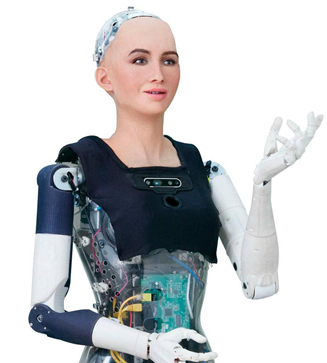
\includegraphics[width=0.6\linewidth]{Main/Chapter2/Images2/Robot-humanoideSophiaIA.png}
        \caption{Robot humanoide Sophia, IA}
        \label{f:Cap2_general_1}
    \end{figure}   
    
    La palabra robot fue usada por primera vez en el año 1921 en la obra de teatro R.U.R (Rossums Universal Robots) creada por el escritor checo Carel Capek (1890 - 1939). El origen etimológico de la palabra es robota, que significa en checo trabajo forzado o esclavo. Posteriormente se emplea la palabra "robótica" en obras de ciencia ficción tales como: Yo Robot (1950) y Robots e imperio (1985) creadas por el escritor y profesor de bioquímica Isaac Asimov (1920-1992).
    
    \begin{figure}[htb]
        \centering
        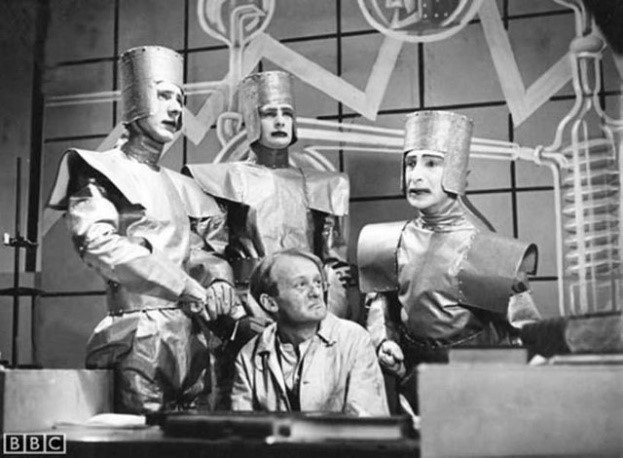
\includegraphics[width=0.4\linewidth]{Main/Chapter2/Images2/Obra-robots.jpg}
        \caption{Obra R.U.R (Robots Universal Rossum) creada por Karel Capek}
        \label{f:Cap2_general_2}
    \end{figure}
    
    Hoy en día los expertos en el área de la robótica y automatización no han llegado a un acuerdo para una definición universal de la palabra robot. Es por esta razón que a continuación se presenta la descripción de un robot respecto al punto de vista de tres instituciones importantes:
    
    \begin{itemize}
    
        \item \textbf{Robot Institute of America (RIA)}: \"Un robot es un manipulador reprogramable multifuncional diseñado para mover material, partes, herramientas o dispositivos especializados a través de movimientos programados variables para el desarrollo de una variedad de tareas.\"
        
        \item \textbf{Japanese Industrial Robot Association (JIRA)}: "Un robot de un dispositivo con grados de libertad que puede ser controlado."
        
        \item \textbf{International Federation of Robotics (IFR)}: "Un robot es un mecanismo actuado programable en dos o más ejes con un grado de autonomía, que se mueva en su entorno para realizar tareas previstas.\\
        \textit{Nota 1: Un robot incluye el sistema de control y la interfase con el sistema de control.}\\
        \textit{Nota 2: La clasificación de robot industrial o robot de servicio se hace de acuerdo con la aplicación prevista.}
        
    \end{itemize}
    
    A parir de las tres definiciones anteriores podemos concluir que un robot es un mecanismo programable o re-programable, capaz de interactuar con acciones independientes e inteligentes en un entorno especifico para realizar una variedad de tareas previstas.
    
    En este trabajo de título se estudia un robot de tipo delta. Esta compuesto por tres brazos conectados a una base fija y a otra móvil llamada efector. Al estar los tres brazos conectados a la misma base, la cinemática del robot es cerrada. Los brazos se accionan por medio de actuadores que generalmente son motores. En el efector final se encuentra generalmente herramientas para realizar tareas especificas.
    
    \begin{figure}[htb]
        \centering
        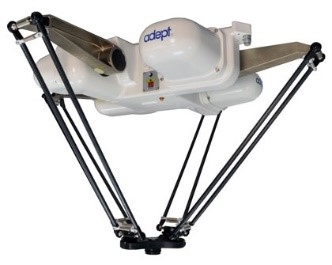
\includegraphics[width=0.4\linewidth]{Main/Chapter2/Images2/Robot-delta-empresa-Adept.jpg}
        \caption{Robot delta empresa Adept}
        \label{f:Cap2_general_3}
    \end{figure}
    
    
\section{Historia de la robótica}
    
    Los robots son una gran noticia hoy en día gracias a las enormes mejoras que han provisto en diversas áreas de la vida de las personas y han abierto un nuevo capítulo en la interacción de humanos y robots para el futuro. Estas enormes mejoras han sido paulatinas, ya que la robótica tiene sus origenes hace miles de años. A continuación, se presentan algunos de los hitos registrados a través de la historia, que han ayudado a la robótica a convertirse en lo que es hoy.
    
\begin{table}[H]
    \centering
    \begin{tabular}{|c|m{12cm}|}
    \hline
        \textbf{Simbología}  & \multicolumn{1}{c|}{\textbf{Descripción}}  \\\hline
         \textbf{400 A.C} & El matemático y filósofo italiano Arquitas de Tarento hizo una paloma de madera que volaba. \\ \hline
         \textbf{10-70 D.C} & El matemático y científico griego Herón de Alejandría construyó diversos autómatas con forma de ave. Se le atribuye la invención de la primera máquina de vapor, conocida como “aeolipile” y la fuente de Herón. \\ \hline
         \textbf{1452 - 1519} & Leonardo Da Vinci diseño 2 autómatas, el primero consiste en un mecanismo que emulaba el movimiento humano vestido de armadura y el segundo un león mecánico \\ \hline
         \textbf{1947} & Primer manipulador eléctrico servo-controlado, por Goetz. \\ \hline
         \textbf{1952} & Primera máquina de control numérico, que se programa por un lenguaje simbólico Software. \\ \hline
         \textbf{1954} & El primer Robot: manipulador tipo brazo articulado que realizaba una secuencia de movimientos programables, desarrollado por George Devol. \\ \hline
         \textbf{1959} & George Devol conoció a Joseph Engelberger y juntos fundaron en 1960 la empresa Unimation dedicada a la fabricación de robot \\ \hline
         \textbf{1960} & Se produce el primer robot de configuración cilíndrica Versatran, por la compañía American Machine Foundry (AMF) \\ \hline
         \textbf{1961} & Unimation instala el primer Unimate en General Motors en los procesos de fundición; mientras que la Ford Motor Company instala un robot Versatran. \\ \hline
         \textbf{1963} & La compañía Fuji Yusoki Kogyo de Japón desarrolla el primer robot para aplicaciones de palletzing, llamado Palletizer. \\ \hline
         \multirow{2}{*}{\textbf{1968}} & Kawasaki adquiere los derechos de fabricación del Unimate en Japón. Comienza la fabricación e implementación de robots en las industrias de Japón. \\ \hline
          & General Motors emplea baterías de robots en el proceso de fabricación de las carrocerías de los coches.\\ \hline
         \textbf{1970} & KUKA, empresa alemana, instala la primera línea de soldadura equipada con robots industriales. \\ \hline
         \textbf{1971} & Se funda la Japanese Industrial Robot Association (JIRA). \\ \hline
         \multirow{2}{*}{\textbf{1973}} & ASEA, empresa sueca, comercializa el primer robot industrial completamente eléctrico, IRB6. \\ \hline
          & La empresa KUKA Robotics contruye el primer robot articulado electromecánicamente de 6 ejes nombrado FAMULUS.\\ \hline
         \textbf{1974} &  \\ \hline
         \textbf{1970} &  \\ \hline
         \textbf{1970} &  \\ \hline
         \textbf{1970} &  \\ \hline
         \textbf{1970} &  \\ \hline
    \end{tabular}
    \caption{Caption}
    \label{tab:my_label}
\end{table}


    
\section{Clasificaciones de robots}
    Desde

    
    
    
\section{Estadísticas y aplicaciones}
    Desde
    
